\documentclass{article}
\usepackage{ben-basic}
\title{Effective Text Editing}
\begin{document}
\pdfbookmark[section]{Contents}{toc}
%\shorttoc{Contents}{1}
\tableofcontents
\clearpage
\section{Literature}
The most basic unit of textual information is not a letter, nor a word, but a sentence.  A letter or word are only supplemental by themselves, and if they hold any inherit meaning, it is only because they are implying a relative sentence.

A sentence is a standard grammatical formation of a statement, which (as it suggests) expresses some state.  Without state there is no activity, and without activity, no life.  Therefore, all proper writing is the conveyence of state colocation and transformation, within a given context.  The mastery of processing both sides of literature (e.g., reading, writing) is condusive to productivity as the requirements of complex engagements have either been resolved or a resolution thereof can be captured in text for posterity.

\section{Latex}
\subsection{Custom Styles}
To prevent the having to copy styles to each latex project on the same host, simply add the style to a texmf (i.e., Tex Metafont) directory, and register it by running the following commands:
mkdir -p ~/texmf/tex/latex
cp <your custom style> ~/texmf/tex/latex
texhash

%TODO credit https://www.ias.edu/math/computing/faq/local-latex-style-files

\section{Git}
\subsection{Authentication Method Ranking}
There are three main options for establishing authentication for write actions like a "push" with a Git.  My criteria for considering both security and productivity results in the following preference order: SSH, password access tokens, password client managers.  SSH is always my first choice, because it offers great convenience and high security standards with the use of the latest RSA public-key encryption.  Yet, some network environments may not allow SSH throughput, therefore "password access tokens" can be used against HTTPS with minimal effort.  As far as password manager clients, it nearly goes without saying that the cumbersome aspect of installing more software to config and set up is not compelling, although, it may offer better security of HTTPS if your current file system is secure.
\subsubsection{SSH}

\subsubsection{Password Access Tokens}

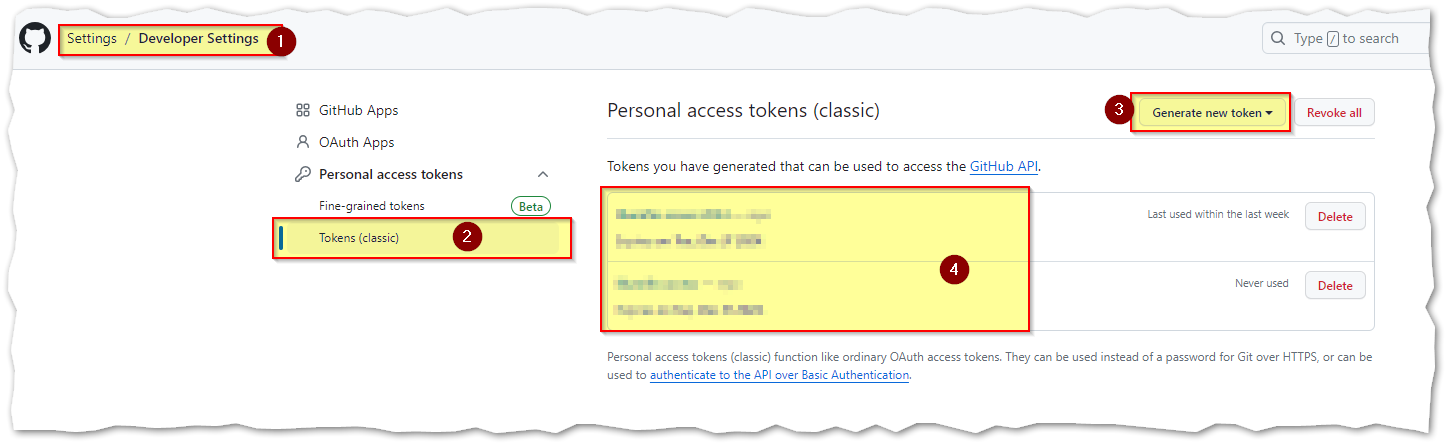
\includegraphics[width=200px]{images/Personal-Access-Tokens.png}
git config credential.helper 'store [<options>]'
\end{document}
